\message{ !name(assignment4.tex)}\documentclass[a4paper]{article}

\usepackage[english]{babel}
\usepackage[utf8]{inputenc}
\usepackage{amsmath}
\usepackage{graphicx}
\usepackage{listings}

\title{Assignment 4}

\author{Axel Goteman and Vilhelm Roxling}

\date{\today}

\begin{document}

\message{ !name(assignment4.tex) !offset(-3) }

\maketitle

\begin{enumerate}

\item{Task 1}

In the first task we observed that the eigenvalue probability distribution seemed to approach a rectangular form from -1 to 1. Why we drew this conclusion is explained by figure \ref{fig: t1a1}.

\begin{figure}
\centering
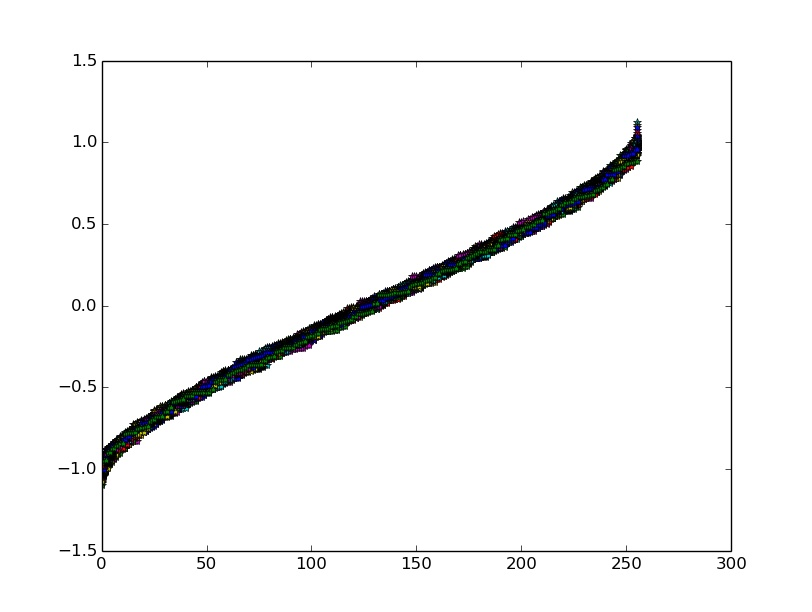
\includegraphics[scale=0.3]{task1_a_1.jpeg}
\caption{\label{fig: t1a1}figtext}
\end{figure} 
Here we have plotted the eigenvalues of 100 256x256 matrices. The eigenvalues are sorted, from smallest to largest, and we can see that they are equally distributed from -1 to 1. For smaller matrices, see figure \ref{fig: t1a2}, 

\begin{figure}
\centering
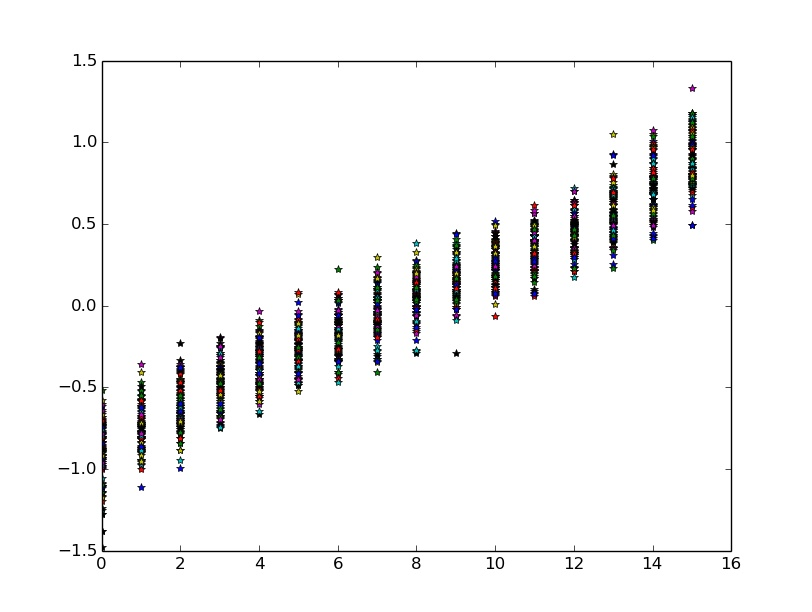
\includegraphics[scale=0.3]{task1_a_2.jpeg}
\caption{\label{fig: t1a2}figtext}
\end{figure} 
the eigenvalues are distributed in the same way but with less strict confinement to the range -1 to 1. I.e the spectral radius $\rho$ converges to 1 for large matrices.

The 2-norm, or the largest singular value, seems to converge to 2, see figure \ref{fig: t1b1}.

\begin{figure}
\centering
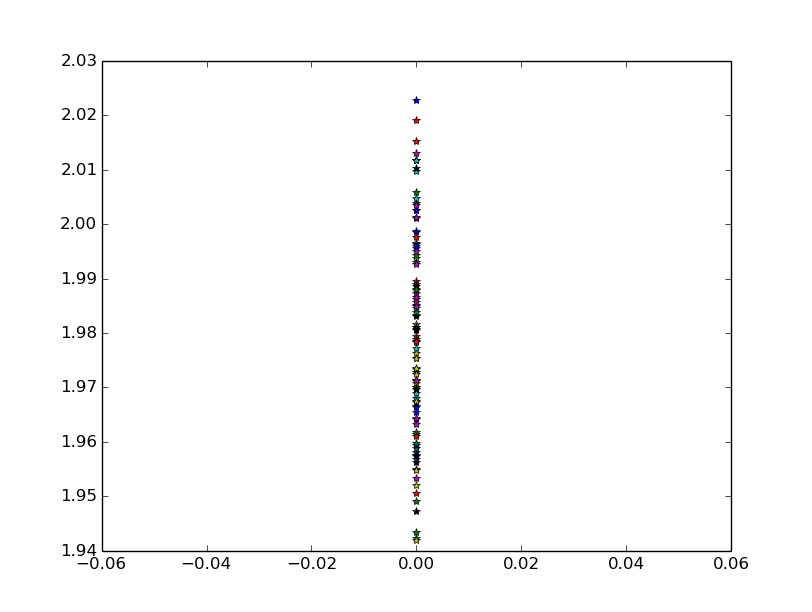
\includegraphics[scale=0.3]{task1_b_1.jpeg}
\caption{\label{fig: t1b1}The 256 eigenvalues sorted for 100 256x256 matrices with normal distributed random elements.}
\end{figure} 

Here $m$=256 and we can see that the average norm is close to 2, and it seems to increase slowly when $m$ grows. 

For a random matrix of size $m$x$m$ the smallest singular value seems to approximately follow the rule $\sigma_{min}\leq(\frac{m}{4})^{-1}=\frac{4}{m}$, i.e the width of the probability distribution close to zero decreases as $\frac{1}{m}$. Or, the probability that a random matrix is very ill-conditioned increases.

For the same distribution of random elements in an upper triangular matrices, the following was observed:

The eigenvalues follows, not unexpectedly, the same distribution as any value of the matrix, obviously because the eigenvalues are found directly on the diagonal. This also means that the spectral radius will converge to zero.

The 2-norm now seems to converge to a value of about 1.6.

For the triangular matrices the smallest singular values converges to zero even faster, the distribution gets narrower at zero and more of the matrices are ill-conditioned.

\item{Task 2}

Using the expanded expression, the achieved result is shown in figure \ref{fig: t21}
\begin{figure}
\centering
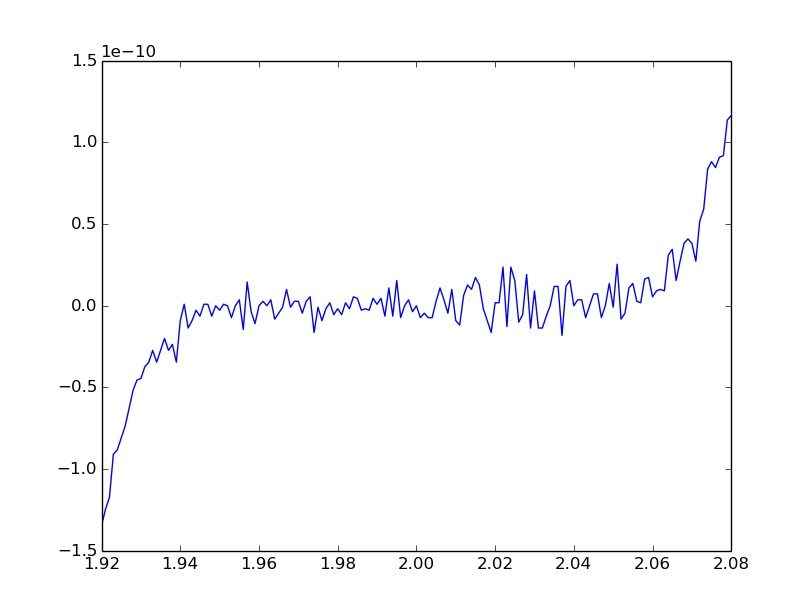
\includegraphics[scale=0.3]{task2_2.jpeg}
\caption{\label{fig: t21}figtext}
\end{figure} 
and the result using the factorized version is shown in figure \ref{fig: t22}
\begin{figure}
\centering
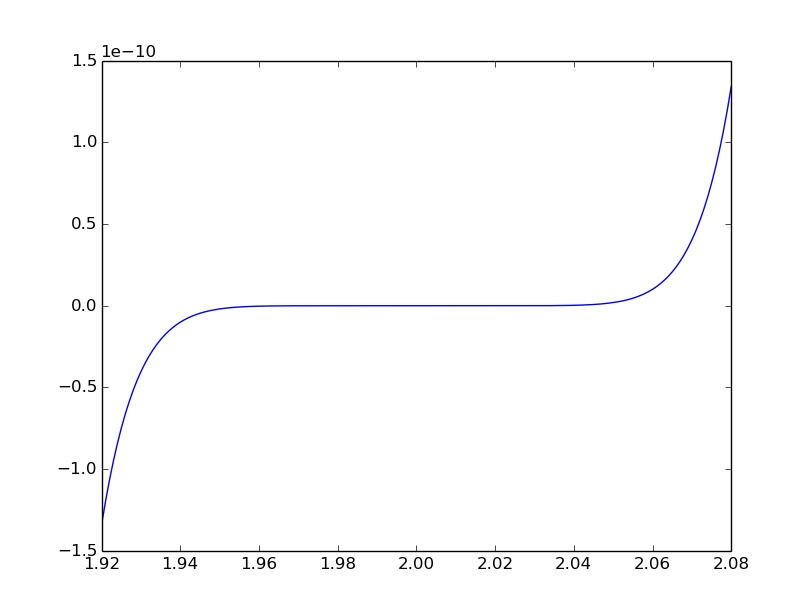
\includegraphics[scale=0.3]{task2_b_1.jpeg}
\caption{\label{fig: t22}figtext}
\end{figure} 
It is easily observed that the expanded version is more sensitive to numerical round off errors.

We suspected that the error was due to operations on larger numbers in the expanded expression resulting in larger round off errors. I.e we suspected that the round off errors were dependent of the size of the number being rounded. In the expanded expression we have numbers in the size of $10^4$, while the factorized are handling numbers of size close to zero. To strengthen this hypothesis we tried to replace the 2 in the factorized expression with 10, and then expand. The error here was several thousand times larger for the expanded expression.

\item{Task 3}
 
We want to find $b$ and $\delta b$ s.t the following holds:
\begin{equation*}
\frac{\|\delta x\|_2}{\|x\|_2}=\kappa_2(A)\frac{\|\delta b\|_2}{\|b\|_2}
\end{equation*}
were $A$ is a full ranked matrix and $\kappa_2(A)=\|A\|_2\|A^{-1}\|_2$ is the condition number of $A$ using the 2-norm. We use the hint that this can be achieved if $b$ and $\delta b$ are expressed in terms of left singular vectors of $A$.

That a vector is left singular vector means that it is an eigenvector to the matrix $AA^T$. If $A=U\Sigma V^T$ is the svd of $A$ then $AA^T=U\Sigma^2U^T$ and $AA^TU = U\Sigma^2$ or $(AA^TU_1 \ldots AA^TU_n)=(\sigma_1^2U_1 \ldots \sigma_n^2U_n)$ where $U_i$ are the columns of $U$. We see directly that the left singular vectors are the columns of $U$. For the two norm we have $\|A\|_2 = \sigma_1$, and $\|A^{-1}\|_2=\frac{1}{\sigma_n}$. This motivates us to choose $b$ and $\delta b$ in terms of the columns of $U$ corresponding to the largest and smallest singular values, i.e $U_1$ and $U_n$. We try with $b = \alpha U_1$ and $\delta b = \beta U_n$. We get by using linearity:
\begin{equation*}
x = A^{-1}b = \alpha V\Sigma^{-1}U^Tb = \alpha V\Sigma^{-1}(1, 0, \ldots 0)^T = \alpha V(\frac{1}{\sigma_1}, 0, \ldots 0)^T = \alpha \frac{V_1}{\sigma_1}
\end{equation*} 
and 
\begin{equation*}
\delta x = A^{-1}\delta b = \beta V\Sigma^{-1}U^Tb = \beta V\Sigma^{-1}(0, \ldots 0, 1)^T = \beta V(0, \ldots 0, \frac{1}{\sigma_n})^T = \beta \frac{V_n}{\sigma_n}
\end{equation*}
Where $V_1$ and $V_n$ is the first respectively the last columns of $V$.Then $\|x\|_2 = \frac{|\alpha|}{\sigma_1}$ and $\|\delta x\|_2 = \frac{|\beta|}{\sigma_n}$ and  
\begin{equation*}
\frac{\|\delta x\|_2}{\|x\|_2}=\frac{|\beta|}{|\alpha|}\frac{\sigma_1}{\sigma_n}
\end{equation*}
\begin{equation*}
\kappa_2(A)\frac{\|\delta b\|_2}{\|b\|_2}=\|A\|_2\|A^{-1}\|_2\frac{\|\beta U_n\|_2}{\|\alpha U_1\|} =\frac{\sigma_1}{\sigma_n}\frac{|\beta|}{|\alpha|}
\end{equation*}
We have equality.

\item{Task 4}

To verify our results in Task 3 we used the code shown below
\begin{lstlisting}
n = 10

A = hilbert(n)
Ainv = invhilbert(n)
# A = np.random.rand(n,n)
# Ainv = np.linalg.inv(A)

u, s, v = svd(A)

alpha = 1
beta = 1e-6

b = alpha*u[:,0]
db = beta*u[:,-1]

x = dot(Ainv, b)
xh = dot(Ainv, b + db)
dx = xh-x

k1 = norm(Ainv, ord=2)*norm(b)/norm(x)
k2 = norm(Ainv, ord=2)*norm(A, ord=2)
k3 = s[0]/s[-1]
k4 = cond(A, p=2)
kv1 = norm(dx)/norm(x)
kv2 = norm(db)/norm(b)

print k1
print k2
print k3
print k4
print kv1/kv2
\end{lstlisting}
We here check the equality of $\kappa_2(A)$ and $\frac{\frac{\|\delta x\|_2}{\|x\|_2}}{\frac{\|\delta b\|_2}{\|b\|_2}}$ when $b$ and $\delta b$ are choosen according to Task 3. We calculate $\kappa_2(A)$ in four different ways, and gets equality for all four with random matrices. With the Hilbert matrix though, we only get equality for size up to about 10. Then the condition number grows much faster than the quota. When using $\kappa_2(A) = \|A^{-1}\|_2\frac{\|b\|_2}{\|x\|_2}$ equality holds to about size 15. But more importantly, our choice of $b$ and $\delta b$ resulted in the quota $\frac{\frac{\|\delta x\|_2}{\|x\|_2}}{\frac{\|\delta b\|_2}{\|b\|_2}}$ being massive. 

\end{enumerate}

\end{document}
\message{ !name(assignment4.tex) !offset(-145) }
